%!TEX root = ../SciVis.tex
\subsection{Skeleton compilation}
\subsection{Color mapping}


understand and implement a set of color mapping techniques for the fluid flow simulation

three datasets: The fluid density rho, the fluid velocity magnitude | v | fig:velocityZebra, and the force field magnitude | f | \ref{fig:forceScaled}

\ref{fig:rainbowColormap}
lookup table

color interpolation

how to specify a colormap
parameterization of colormap (hue and saturation) \ref{fig:saturationAndHueColormap}

defined colormaps \ref{fig:colormaps}
 
vertex vs texture

transform (linear or logarithmic)

banding 

legend  The legend should show both the colormap and the corresponding numerical values associated to various colors.

scaling: the entire actual range (min..max) of the dataset at the current time moment is mapped to the visible colormap. This means, of course, that you have to update the numerical values displayed along with the color legend.
\ref{fig:forceScaled}

clamping: the data values are clamped between two user-prescribed min and max values. These values correspond to the entire range of your color legend. Actual data values higher than min, or lower than max, are actually clamped to min and max respectively. The user should be allowed to change min and max interactively, e.g. by means of some sliders or similar widgets.
 
\begin{figure}[htbp]
    \centering
    \begin{tabular}{ccccccc}
    
\includegraphics[height=2in]{figures/colormaps/grayscale.png}&
      
\includegraphics[height=2in]{figures/colormaps/rainbow.png}&
      
\includegraphics[height=2in]{figures/colormaps/heatmap.png}&         
     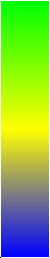
\includegraphics[height=2in]{figures/colormaps/blueYellowGreen.png}&
      
\includegraphics[height=2in]{figures/colormaps/blackGradient.png}&
      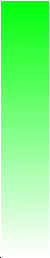
\includegraphics[height=2in]{figures/colormaps/whiteGradient.png}&
      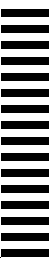
\includegraphics[height=2in]{figures/colormaps/zebra.png}\\
    (a)&(b)&(c)&(d)&(e)&(f)&(g)\\
    \end{tabular}
    \caption{Predefined colormaps: (a) Luminance, (b) Rainbow, (c) Heatmap, (d)  Blue-Green-Yellow, (e) Black Gradient (f) White Gradient (g) Zebra}
    \label{fig:colormaps}
\end{figure}



\begin{figure}[htbp]
\centering
\begin{minipage}[t]{0.48\textwidth}
        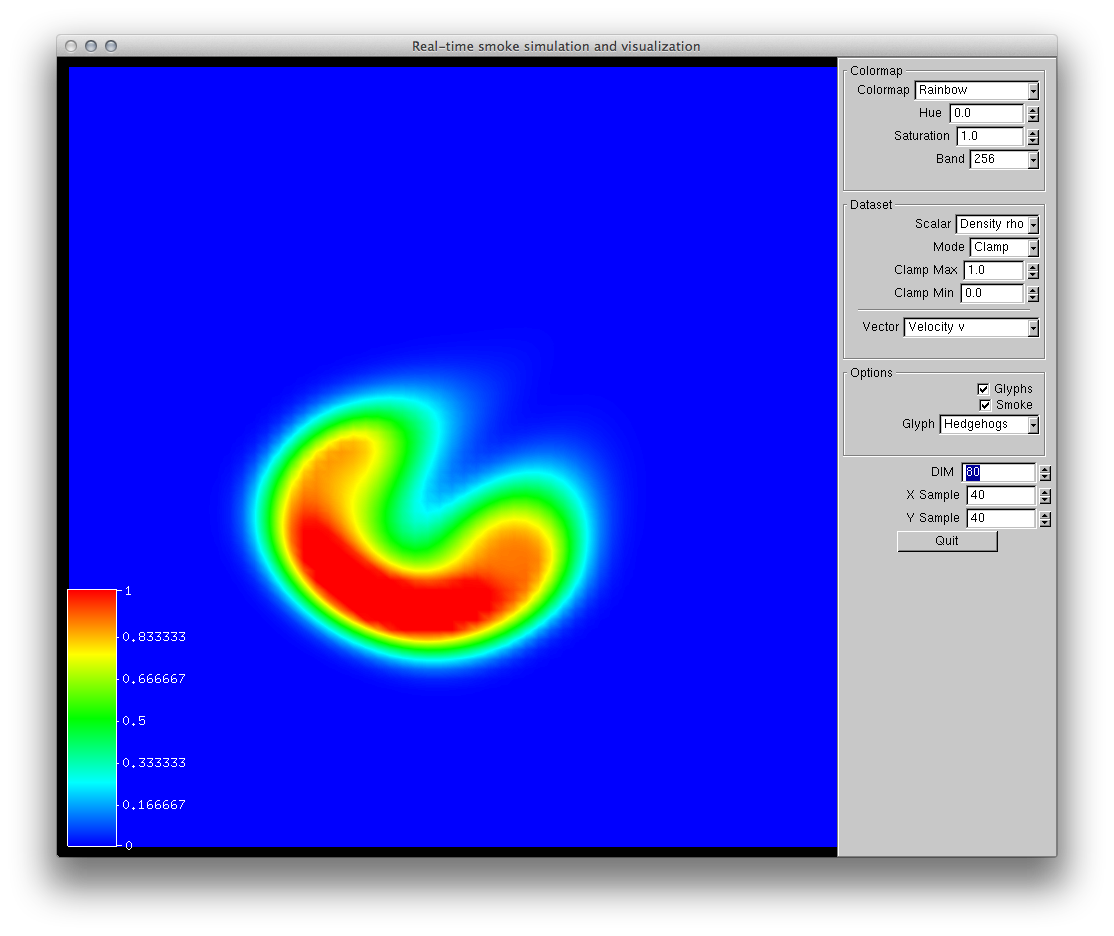
\includegraphics[height=3in]{figures/colormaps/rainbowSmoke.png}
\caption{Fluid density visualized with a rainbow colormap.}
\label{fig:rainbowColormap}
\end{minipage}\hspace{.04\textwidth}%
\begin{minipage}[t]{0.48\textwidth}
        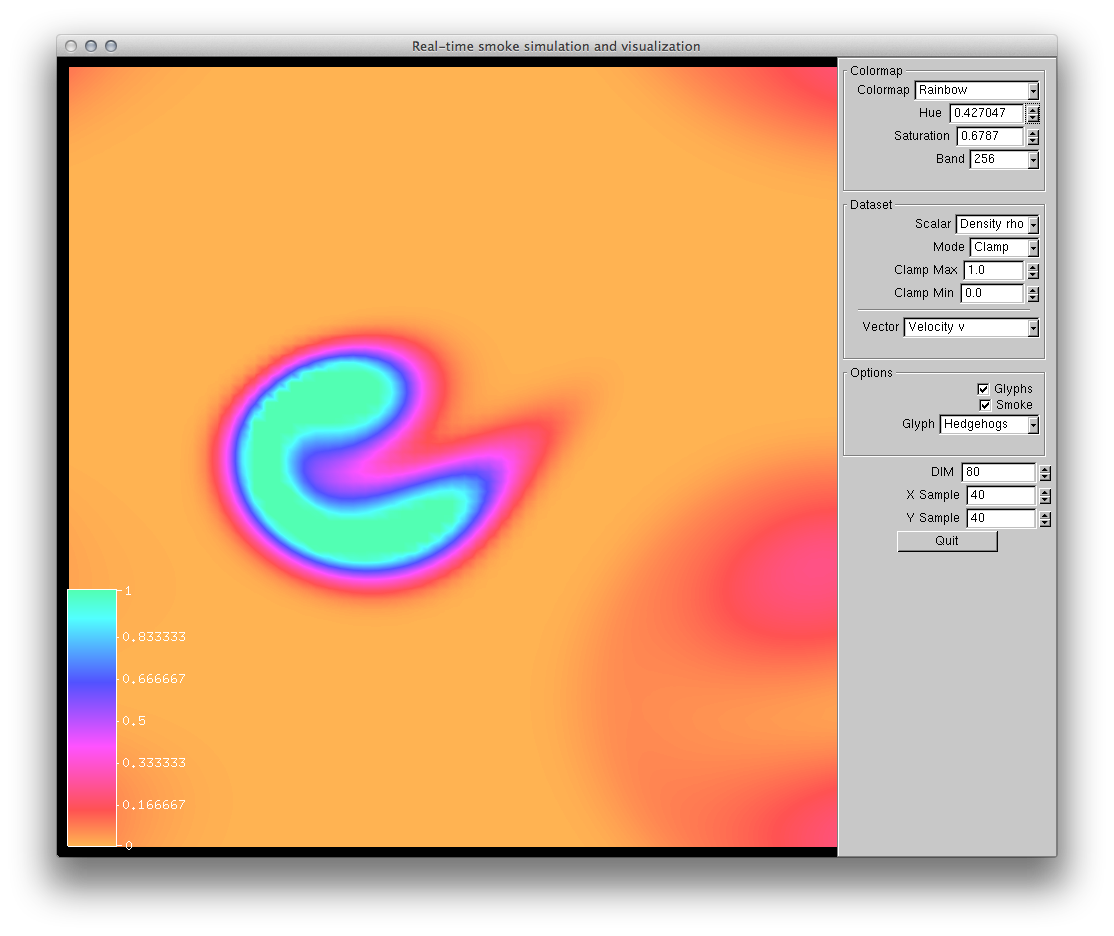
\includegraphics[height=3in]{figures/colormaps/hueAndSaturation.png}
    \caption{Fluid density with a less-saturated and hue-shifted rainbow colormap.}
    \label{fig:saturationAndHueColormap}
\end{minipage}
\end{figure}


\begin{figure}[htbp]
\centering
\begin{minipage}[t]{0.48\textwidth}
        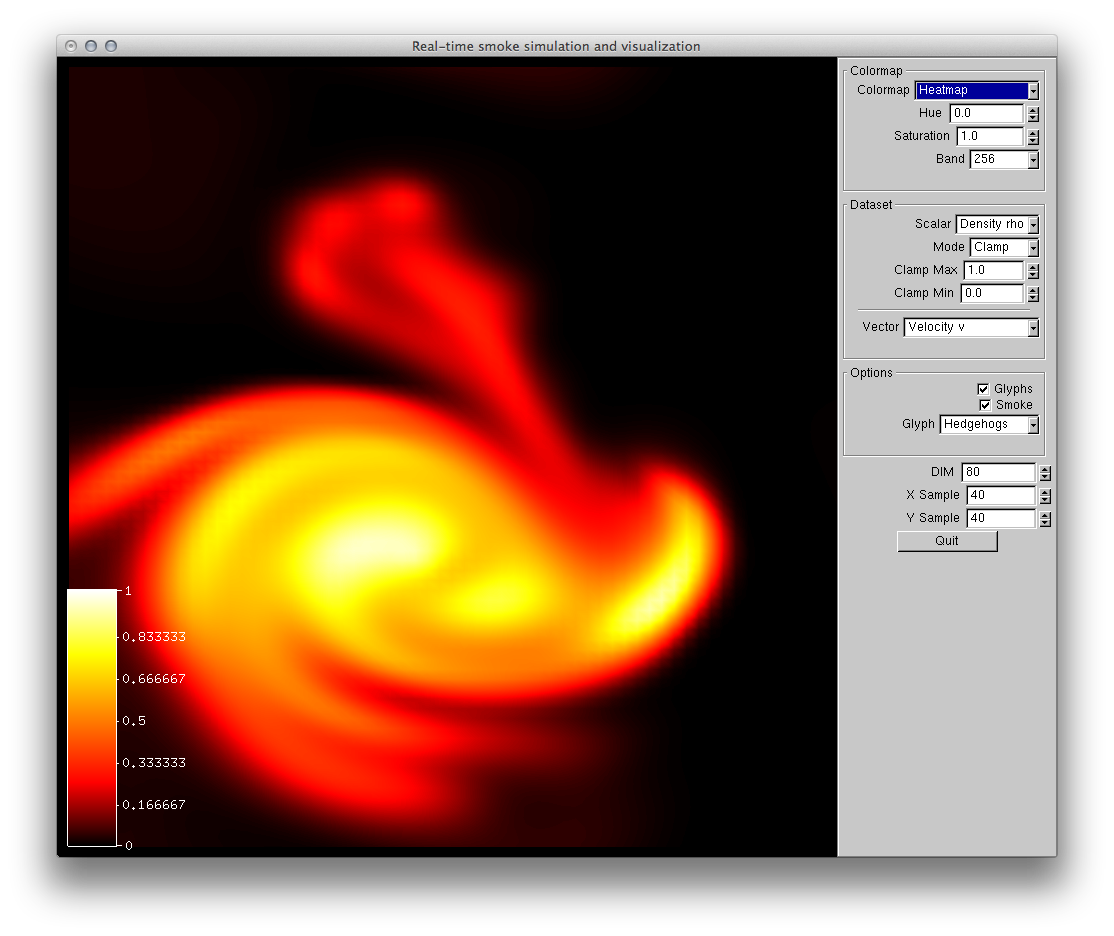
\includegraphics[height=3in]{figures/colormaps/heatmapSmoke.png}
\caption{Fluid density visualized with a heat colormap}
\label{fig:revised:modelingLanguages}
\end{minipage}\hspace{.04\textwidth}%
\begin{minipage}[t]{0.48\textwidth}
        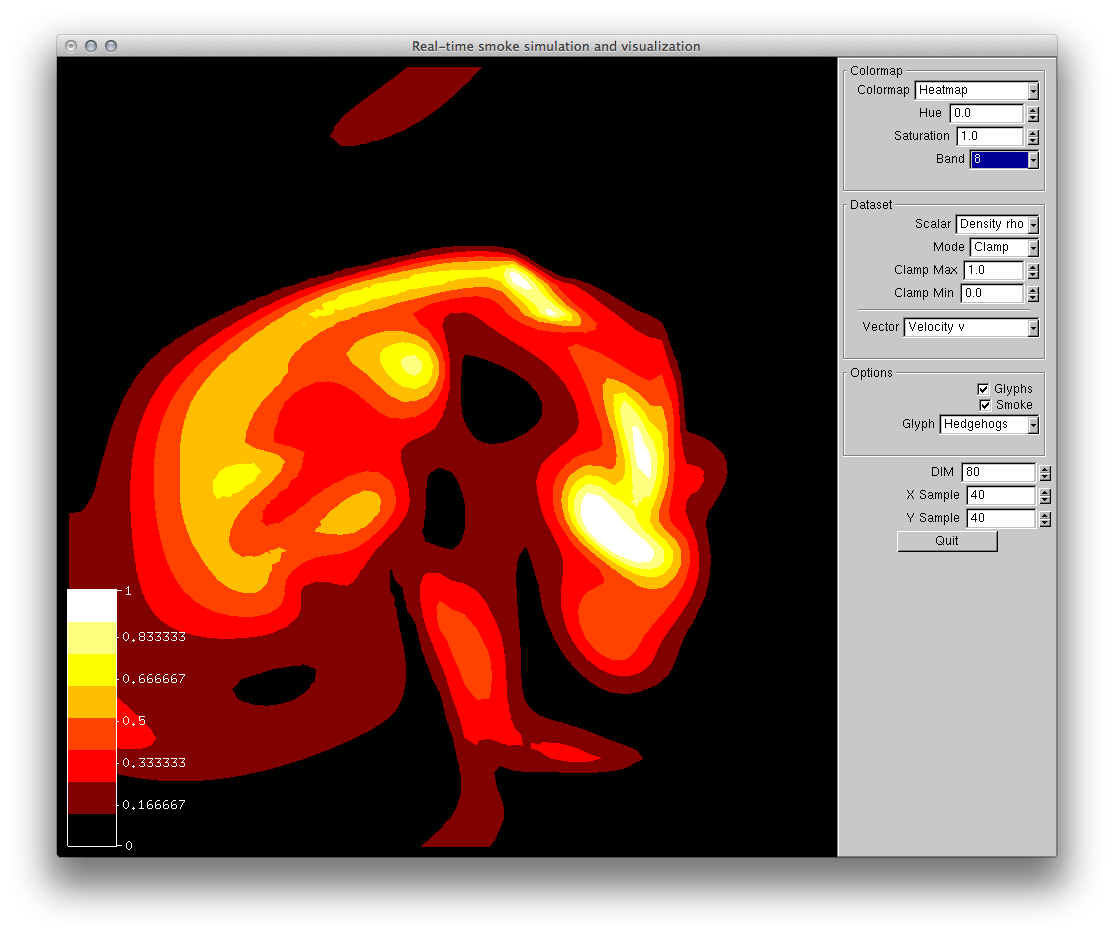
\includegraphics[height=3in]{figures/colormaps/heatmapSmokeBanded.png}
    \caption{Heat colormap with a reduced number of colors. The color banding effect is clearly visible.}
    \label{fig:revised:reqFormat}
\end{minipage}
\end{figure}

\begin{figure}[htbp]
\centering
\begin{minipage}[t]{0.48\textwidth}
        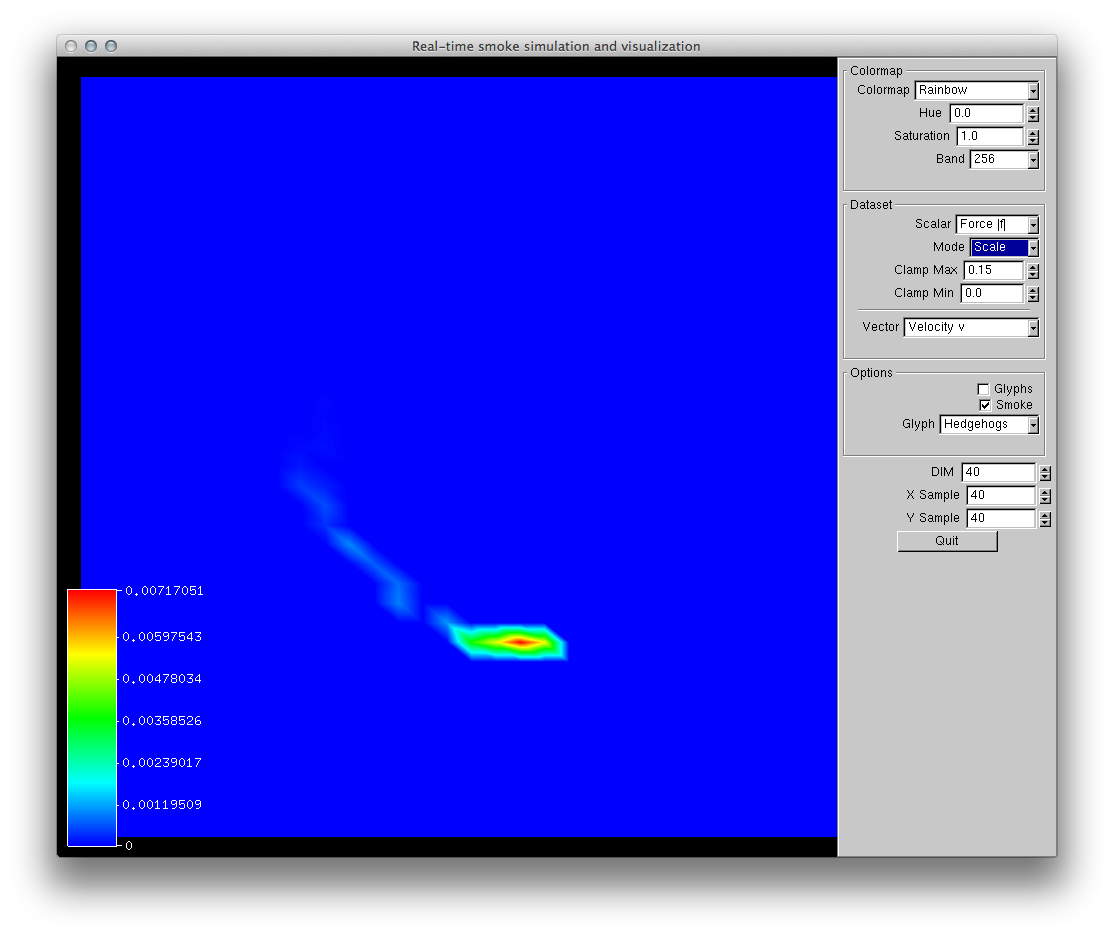
\includegraphics[height=3in]{figures/colormaps/forceScaled.png}
\caption{Scaling the colormap to the min and max of force always shows the maximum and minimum values at the current timestep although the values are quite small.}
\label{fig:forceScaled}
\end{minipage}\hspace{.04\textwidth}%
\begin{minipage}[t]{0.48\textwidth}
        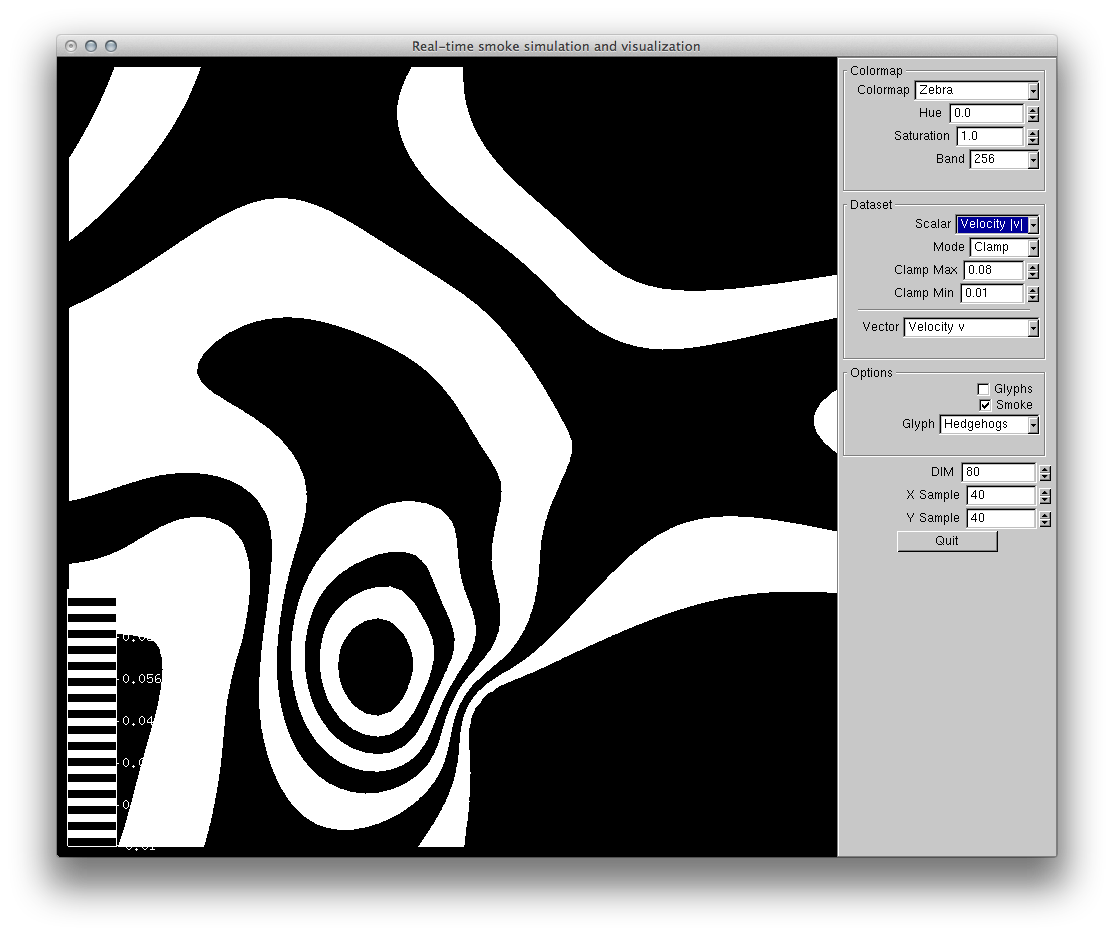
\includegraphics[height=3in]{figures/colormaps/velocityZebra.png}
    \caption{Velocity visualized with a zebra colormap that highlights areas with high variation.}
    \label{fig:velocityZebra}
\end{minipage}
\end{figure}


\subsection{Glyphs}


The aim of this step is for you to understand and implement a set of glyph techniques. Glyphs are icons that convey the value (orientation, magnitude) of a vector field by means of several graphical icons, such as arrows. Glyphs can also be used to visualize several types of fields together, such as one scalar field and one vector field, at the same spatial locations. In this step, you will design and implement several glyphs for visualizing three datasets: The fluid density rho, the fluid velocity v, and the force field f. For a description of these quantities, see the skeleton code.
 
There is already a very basic implementation of arrow glyphs, also known as hedgehogs, provided in the skeleton code. Using this implementation as a starting point, and also the material in the book and lectures, you have to implement yourself several new functionalities, as follows.
 
·        Implement a mechanism that lets you choose one scalar field and one vector field and visualizes their combination using glyphs. As scalar fields, you should be able to choose from: the density rho, the fluid velocity magnitude | v |, and the force field magnitude | f |. These are exactly the scalar fields used at step 2. As vector fields, you should be able to choose from: fluid velocity v and the force field f. Use the vector field direction and magnitude to control the orientation and length (respectively) of the arrows. Use the scalar field to control the arrows’ colors. For this, use the color map techniques designed at step 2.
 
·        Implement a mechanism to specify where to draw the glyphs. Start by modifying the mechanism currently implemented in the code which places the glyphs on a regular sampling of the grid. Provide interactive controls to specify the number of samples, in the x and y directions, where you want to evaluate the vector field. In case your sample points do not coincide with an actual computational grid point, provide interpolation mechanisms that compute the dataset values out of the grid neighbour point(s). Here, you can choose between nearest-neighbor (constant) and (bi)linear interpolation.
 
·        Implement a mechanism that lets you parameterize the glyph itself. Besides using simple two-dimensional arrows (hedgehogs), implement two other glyph types that are able to show both a vector field and a scalar field. Suggestions include, but are not limited to:
 
three-dimensional cones
three-dimensional ellipsoids
three-dimensional arrows consisting of a cone tip and a cylindrical shafts
arrows implemented as two-dimensional nice-looking, high-quality, textures instead of simple polygonal shapes
 
Just as for the previous steps, provide interactive means to choose the datasets and types of glyphs at runtime. Consider carefully the glyph design: How thick to make the glyph? How long to make it? Should you scale the length linearly with the vector magnitude, or use another scale? Should you clamp the glyph’s minimal and maximal sizes to some values? If so, which are those?

\begin{figure}[htbp]
\centering
\begin{minipage}[t]{0.48\textwidth}
 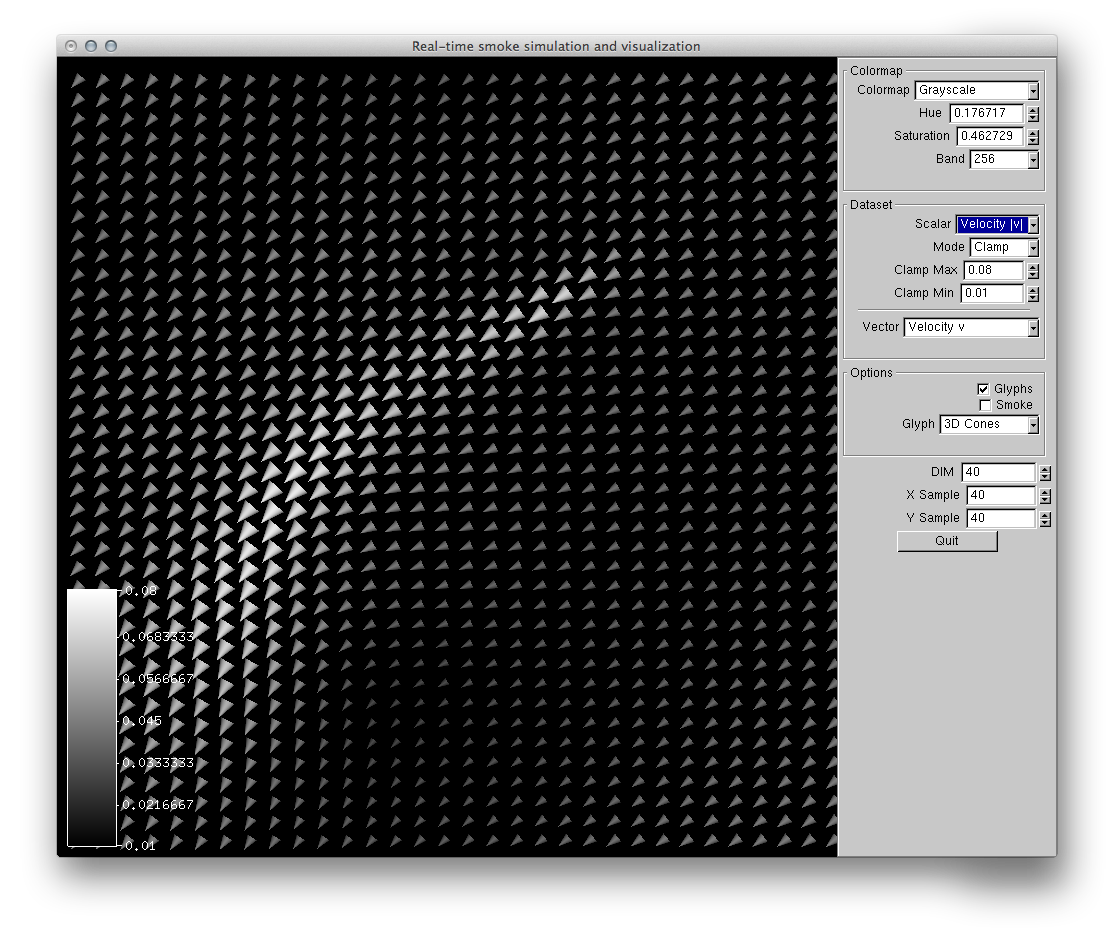
\includegraphics[height=3in]{figures/glyph/conesVelocityGrayscale.png}
\caption{}
\label{fig:forceScaled}
\end{minipage}\hspace{.04\textwidth}%
\begin{minipage}[t]{0.48\textwidth}
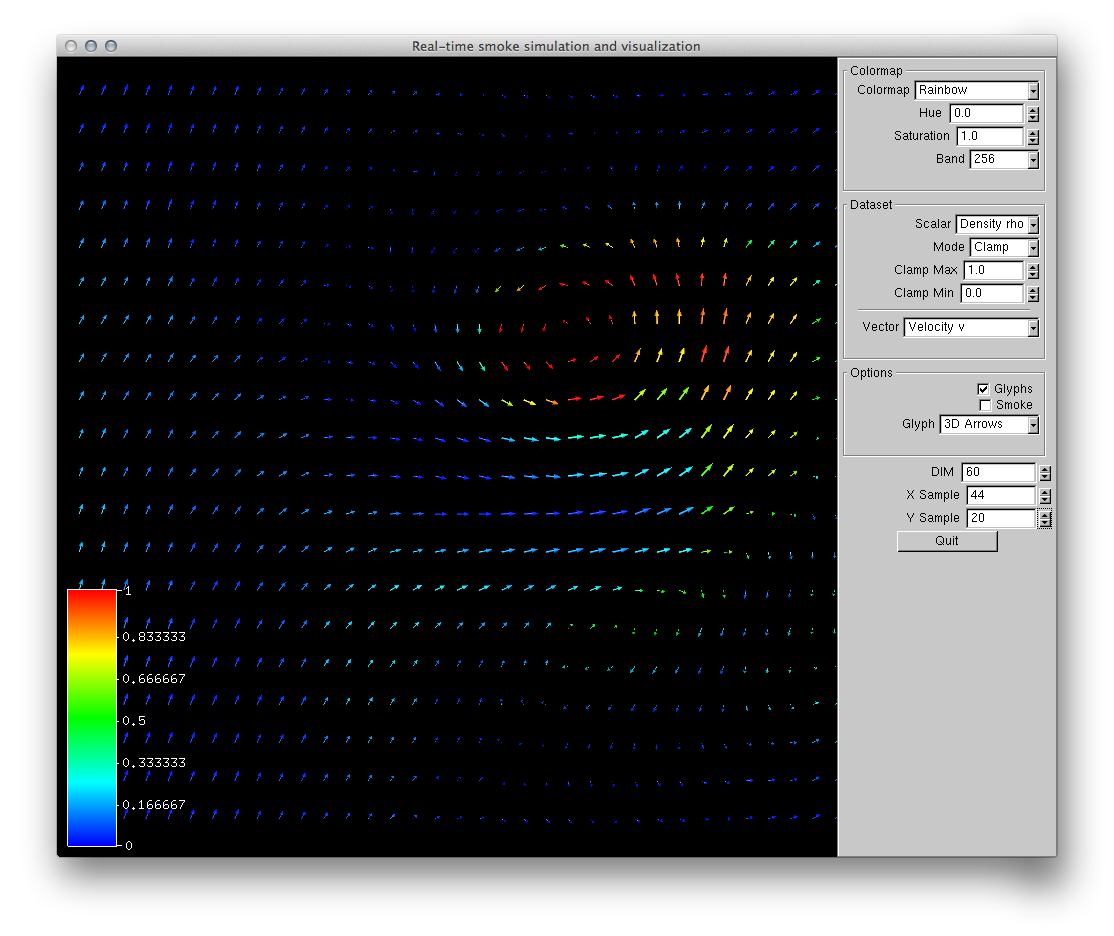
\includegraphics[height=3in]{figures/glyph/arrowsDensityVelocityRainbow.png}
    \caption{}
    \label{}
\end{minipage}
\end{figure}


\subsection{Gradient}
\subsection{Streamlines}
\subsection{Slices}
\subsection{Stream surfaces}